% Compile with:
% latexmk -lualatex -pvc -interaction=nonstopmode 20220629_MICResearchDay.tex
%\documentclass[aspectratio=169,draft]{beamer}
\documentclass[aspectratio=169]{beamer}
\usetheme{UniBern}

\title{micro-CT imaging across scales and faculties}
\author{David Haberthür}
\date{June 29, 2022 | \href{https://www.mic.unibe.ch/events/mic_research_day_2022}{MIC Research Day 2022}}

\includeonlyframes{current}
%then....
%\begin{frame}[label=current]
%\end{frame}

\usepackage[detect-all=true,
	binary-units=true,
	per-mode=symbol,
	per-symbol=/]{siunitx}
\usepackage{xspace}
\usepackage{gitinfo2}
\usepackage[backend=biber,
	style=numeric,
	url=false,
	maxnames=1,
	sorting=none,
	]{biblatex}
\addbibresource{/home/habi/P/Documents/library.bib} % anaklin25
%\addbibresource{/Users/habi/Documents/library.bib} % anomalocaris
\usepackage{ccicons}
\usepackage{animate}
\usepackage{tikz}
	\usetikzlibrary{shadows,mindmap}
	\tikzset{shadowed/.style={preaction={transform canvas={shift={(1pt,-1pt)}},draw=ubRed}}}
\usepackage{shadowtext} % for the shadowed scalebar
	\shadowoffset{1pt}
	\shadowcolor{ubRed}
\usepackage{environ}
\usepackage[absolute,overlay]{textpos} % for the \source* command
\usepackage{fontawesome5}
\usepackage{emoji}
\usepackage{listings}
	\lstset{frame=single,
	basicstyle=\tiny\ttfamily
	}
\usepackage{booktabs}
\usepackage{multirow}
\usepackage{colortbl}
\usepackage{adjustbox}
\usepackage{microtype}

% Some often used abbreviations/commands
\newcommand{\everyframe}{25} % use only every nth frame for the animations
\newcommand{\imwidth}{\linewidth}% set global image width
\newcommand{\imheight}{0.725\paperheight}% set global image height
\newlength\imagewidth% needed for scalebars
\newlength\imagescale% needed for scalebars
\newcommand{\uct}{\textmu CT\xspace}% make our life easier
\newcommand{\eg}{e.\,g.\xspace}%
\newcommand{\ie}{i.\,e.\xspace}%

% Define complementary colors to ubRed
\definecolor{ubRedComplementary1}{HTML}{00a1e6}
\definecolor{ubRedComplementary2}{HTML}{00e645}

% Acknowledge images just below them
% Based on https://tex.stackexchange.com/a/282637/828
\newcommand{\source}[2]{%
	% Print out (short) link under image, with small text
	\raisebox{-1.618ex}{%
		\makebox[0pt][r]{%
			\scriptsize\href{http://#1}{#1} #2%
			}%
		}%
	}%
\newcommand{\sourcecite}[2]{%
	% Cite (an image from) a reference
	\raisebox{-1.618ex}{%
		\makebox[0pt][r]{%
			\scriptsize From \cite{#1}, #2%
			}%
		}%
	}%
\newcommand{\sourcelink}[3]{%
	% Make the source command an \href{link}{text}
	\raisebox{-1.618ex}{%
		\makebox[0pt][r]{%
			\scriptsize\href{http://#1}{#2}, #3%
			}%
		}%
	}%
% Define us a custom footer *with* progress bar, based on https://tex.stackexchange.com/a/59749/828
\makeatletter
\def\progressbar@progressbar{} % the progress bar
\newcount\progressbar@tmpcounta% auxiliary counter
\newcount\progressbar@tmpcountb% auxiliary counter
\newdimen\progressbar@pbht %progressbar height
\newdimen\progressbar@pbwd %progressbar width
\newdimen\progressbar@rcircle % radius for the circle
\newdimen\progressbar@tmpdim % auxiliary dimension
\progressbar@pbwd=0.85\linewidth
\progressbar@rcircle=1.5pt
\def\progressbar@progressbar{%
	\progressbar@tmpcounta=\insertframenumber
	\progressbar@tmpcountb=\inserttotalframenumber
	\progressbar@tmpdim=\progressbar@pbwd
	\multiply\progressbar@tmpdim by \progressbar@tmpcounta
	\divide\progressbar@tmpdim by \progressbar@tmpcountb
	\par%
	\begin{tikzpicture}%
		\draw[ubGrey] (0,0) -- ++ (\progressbar@pbwd,0);
		\draw[draw=ubRed,fill=ubGrey] (\the\dimexpr\progressbar@tmpdim-\progressbar@rcircle\relax,.5\progressbar@pbht) circle (\progressbar@rcircle);
	\end{tikzpicture}%
	\hfill bit.ly/MICRday\xspace|\xspace%
	v. \href{https://github.com/habi/Talk.2022.MICResearchDay/commit/\gitHash}{\gitAbbrevHash}\xspace|\xspace%
	p.\xspace\insertframenumber/\inserttotalframenumber%
	\hspace*{4ex}%
	\vspace{0.5ex}%
	%\par%
}
\addtobeamertemplate{footline}{}%
{%
	\begin{beamercolorbox}[wd=\paperwidth,center]{green}%
		\progressbar@progressbar%
	\end{beamercolorbox}%
}%
\makeatother

% Format bibliography for beamer
% http://tex.stackexchange.com/a/10686/828
\renewbibmacro{in:}{}
% http://tex.stackexchange.com/a/13076/828
\AtEveryBibitem{%
	\clearfield{journaltitle}
	\clearfield{pages}
	\clearfield{volume}
	\clearfield{number}
	\clearname{editor}
	\clearfield{issn}
	\clearfield{year}
}
% No parentheses around the (now empty) year: https://tex.stackexchange.com/a/147537/828
\renewcommand{\bibopenparen}{\addcomma\addspace}
\renewcommand{\bibcloseparen}{\addcomma\addspace}

% open in fullscreen
%\hypersetup{pdfpagemode=FullScreen}

% Move the whole text area down a bit
% THIS IS A BIG HACK, AND SHOULD BE FIXED IN THE TEMPLATE
\addtobeamertemplate{frametitle}{}{\vspace*{0.71em}}

\begin{document}
% No footline on the title page
% http://tex.stackexchange.com/a/18829/828 helps us to achieve that
{%
	\setbeamertemplate{footline}{}%
	\begin{frame}%
		\maketitle
	\end{frame}%
}

\begin{frame}
	\frametitle{\emph{Grüessech} from the \uct-group}
	\centering
	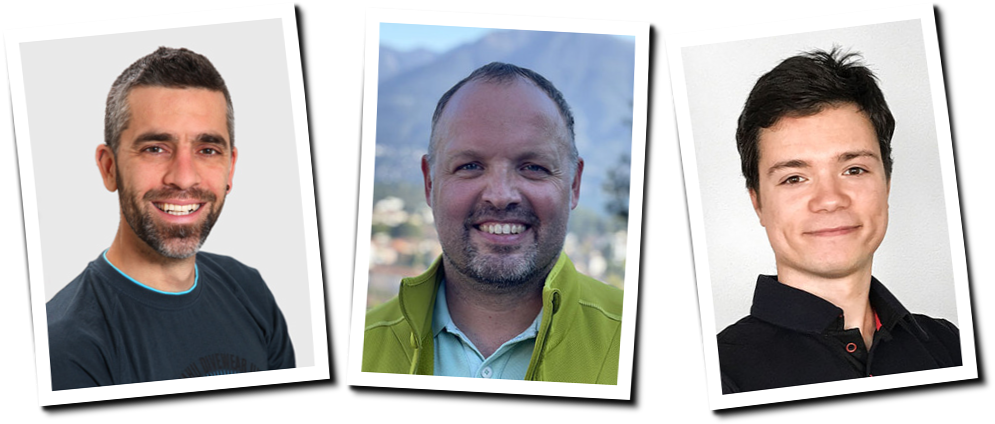
\includegraphics[width=\linewidth]{./images/team}
\end{frame}

\begin{frame}
	\frametitle{LOAFS}
	\uct
	
	Non-destructive imaging across scales
	
	Ich zeige nur \emph{uni-interne} Projekte, wir machen noch (viel) mehr	
\end{frame}

\begin{frame}
	\frametitle{Machinery at the Institute of Anatomy}
	\begin{columns}
		\begin{column}{0.333\linewidth}
			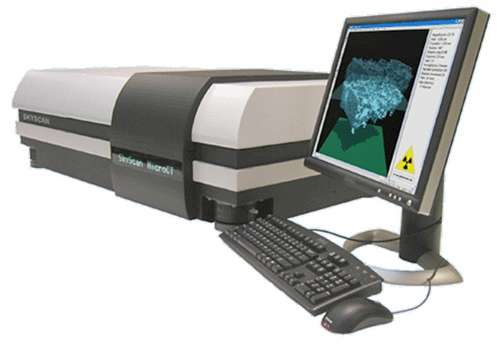
\includegraphics[width=\linewidth]{./images/1172}%
			\source{brukersupport.com}{}
		\end{column}
		\begin{column}{0.333\linewidth}
			\includegraphics<1>[width=\linewidth]{./images/1272}%
			\source{bruker.com/skyscan1272}{}
		\end{column}
		\begin{column}{0.333\linewidth}
			\includegraphics<1>[width=\linewidth]{./images/2214}%
			\source{bruker.com/skyscan2214}{}
		\end{column}							
	\end{columns}
\end{frame}

\begin{frame}
	\frametitle{Overview}
	\centering
	\only<1>{%
		\begin{tikzpicture}%
            \tikzset{small mindmap}%
            \tikzset{level 1 concept/.append style={scale=0.9,level distance = 40mm,transform shape}}%
            \tikzset{level 2 concept/.append style={scale=0.95,level distance = 25mm,transform shape}}%		
		    \path[mindmap,every node/.style={concept,circular drop shadow},concept color=ubRed]%
			    node[concept] {unibe.ch\ Faculties}
				    child [grow=15]  {node[concept] {Business, Economics ​and Social Sciences}}
    				child [grow=45]  {node[concept] {​Law}}
	    			child [grow=135] {node[concept] {​Human Sciences}}
	       			child [grow=165] {node[concept] {​Science}}
	       			child [grow=195] {node[concept] {​Humanities}}	
	    			child [grow=345] {node[concept] {​Medicine}}
    				child [grow=225] {node[concept] {Vetsuisse}}
	    			child [grow=315] {node[concept] {​Theology}};%
		\end{tikzpicture}%
	}%
	\only<2>{%
		\begin{tikzpicture}%
            \tikzset{small mindmap}%
            \tikzset{level 1 concept/.append style={scale=0.9,level distance = 40mm,transform shape}}%
            \tikzset{level 2 concept/.append style={scale=0.95,level distance = 25mm,transform shape}}%
		\path[mindmap,every node/.style={concept,circular drop shadow},concept color=ubRed!31!white,semitransparent]%
			node{unibe.ch\ Faculties}
				child [grow=15]  {node[concept] {Business, Economics ​and Social Sciences}}
				child [grow=45]  {node[concept] {​Law}}
				child [grow=135] {node[concept] {​Human Sciences}}
      				child [concept color=ubRed,opaque,grow=165] {node[concept] {Science}}				
    				child [grow=195] {node[concept] {​Humanities}}							
	    			child [concept color=ubRed,opaque,grow=225] {node[concept] {Vetsuisse}}    				
				child [grow=315] {node[concept] {​Theology}}
				child [concept color=ubRed,opaque,grow=345] {node[concept] {​Medicine}};%
		\end{tikzpicture}%
	}%
	\only<3>{%
		\begin{tikzpicture}%
            \tikzset{small mindmap}%
            \tikzset{level 1 concept/.append style={scale=0.9,level distance = 40mm,transform shape}}%
            \tikzset{level 2 concept/.append style={scale=0.95,level distance = 25mm,transform shape}}%		
		    \path[mindmap,every node/.style={concept,circular drop shadow},concept color=ubRed!31!white,semitransparent]%
			    node{unibe.ch\ Faculties}
			    	child [grow=15]  {node[concept] {Business, Economics ​and Social Sciences}}
			    	child [grow=45]  {node[concept] {​Law}}
			    	child [grow=135] {node[concept] {​Human Sciences}}
    		    		child [grow=195] {node[concept] {​Humanities}}
			    	child [grow=315] {node[concept] {​Theology}}
      		    		child [concept color=ubRed,opaque,grow=165] {node[concept] {Science}
			    		child [concept color=ubRed,opaque,grow=-45] {node[concept] {{Institute of Ecology and Evolution}}}
			    		child [concept color=ubRed,opaque,grow=15]  {node[concept] {Space Research \& Planetary Sciences}}
			    		}
    				child [concept color=ubRed,opaque,grow=225] {node[concept] {Vetsuisse}
    				    child [concept color=ubRed,opaque,grow=0] {node[concept] {Clinical radiology}}
    				    }
				    child [concept color=ubRed,opaque,grow=345] {node[concept] {​Medicine}
					    child [concept color=ubRed,opaque,grow=105] {node[concept] {Theodor Kocher Institute}}
    					child [concept color=ubRed,opaque,grow=140] {node[concept] {School of Dental Medicine}}
	    				child [concept color=ubRed,opaque,grow=185] {node[concept] {Institute of Anatomy}}
	    				child [concept color=ubRed,opaque,grow=225] {node[concept] {Klinik für Orthopädische Chirurgie \& raumatologie}}
	    				};%
		\end{tikzpicture}%
	}%	
\end{frame}

\begin{frame}
	\frametitle{Overview}
	\begin{columns}
		\begin{column}{0.309\linewidth}
			Scales
			\begin{itemize}
				% Get emojis from https://unicode.org/emoji/charts/emoji-list.html
				\item \only<1>{\huge{\emoji{unicorn}}}\only<2>{\huge{\emoji{horse}}}% or \emoji{unicorn} ?
				\normalsize\item \huge{\emoji{peach}}
				\normalsize\item \huge{\emoji{fish}}% or \emoji{tropical-fish} ?
                \normalsize\item \huge{\emoji{mouse-face}}% or \emoji{mouse} ?	
				\normalsize\item \huge{\emoji{tooth}}% or \emoji{tropical-fish} ?
				\normalsize\item \huge{\emoji{comet}}
			\end{itemize}
		\end{column}
		\begin{column}{0.618\linewidth}
			Faculties
			\begin{itemize}
				\item Vetsuisse Faculty
				\begin{itemize}
				    \item Clinical Radiology
				\end{itemize}
				\item Faculty of Science
				\begin{itemize}
					\item Institute of Ecology and Evolution
					\item Space Research \& Planetary Sciences (WP)
				\end{itemize}	
				\item Faculty of Medicine
				\begin{itemize}
					\item Theodor Kocher Institute (TKI)
					\item School of Dental Medicine
					\item Institute of Anatomy
					\item Universitätsklinik für Orthopädische Chirurgie und Traumatologie
				\end{itemize}
			\end{itemize}
		\end{column}
	\end{columns}
\end{frame}

\begin{frame}
	\frametitle{Hoof}%
	\begin{columns}%
		\begin{column}{0.495\linewidth}%
		    Laminitis \cite{Blaettler2022}%
    		Contrast-agent \cite{Hlushchuk2018}%
		\end{column}%
		\begin{column}{0.495\linewidth}%
	        \centering%
            \only<1>{%
                \animategraphics[height=\imheight,every=\everyframe]{24}{./images/VETSUISSE/HorseLimb/Limb02/setup-frames/IMG_69500}{001}{634}%
                }%
            \only<2>{%
                \renewcommand{\imwidth}{1.035738368*\imheight}% 1536/1483    
                \pgfmathsetlength{\imagewidth}{\imwidth}%
		        \pgfmathsetlength{\imagescale}{\imagewidth/1536}%
		        \def\x{949-100}% scalebar-x starting at golden ratio of image width of 1536px = 949
		        \def\y{1335}% scalebar-y at 90% of image height of 1483px = 1335
		        \begin{tikzpicture}[x=\imagescale,y=-\imagescale]%
			        \node[anchor=north west, inner sep=0pt, outer sep=0pt] at (0,0) {\includegraphics[width=\imagewidth]{./images/VETSUISSE/HorseLimb/Limb02/"MAX_Reslice of merged-bin2x"}};
			        % Since we draw the scale bar on the *binned* dataset, each pixel is not 40.999924, but 81.999848 um
			        % 1536.000px = 125.95176652800001mm -> 100px = 8199.985um -> 6.098px = 500um, 1.220px = 100um
			        %draw[|-|,blue,thick] (0,742) -- (1536,742) node [sloped,midway,above,fill=white,semitransparent,text opacity=1] {\SI{125.95}{\milli\meter} (1536px) TEMPORARY!};
			        \draw[|-|,white,thick,shadowed] (\x,\y) -- (\x+609.8,\y) node [midway,above] {\shadowtext{\SI{5}{\centi\meter}}};
		        \end{tikzpicture}%
		        }%
	    \end{column}%
    \end{columns}%
\end{frame}

%Reset image height
\renewcommand{\imheight}{0.725\paperheight}% set global image height
\begin{frame}
	\frametitle{Hoof}
        \centering
		\animategraphics[autoplay,height=\imheight,every=\everyframe]{24}{./images/VETSUISSE/HorseLimb/Limb02/frames/video-0}{000}{300}
\end{frame}

\begin{frame}
	\frametitle{Sakrum}
		\centering
		\only<1>{%
			\renewcommand{\imwidth}{\imheight}% Fortunately, we have square frames here...
			\pgfmathsetlength{\imagewidth}{\imwidth}%
			\pgfmathsetlength{\imagescale}{\imagewidth/1024}%
			\def\x{633}% scalebar-x starting at golden ratio of image width of 1024px = 633
			\def\y{922}% scalebar-y at 90% of image height of 1024px = 922
			\begin{tikzpicture}[x=\imagescale,y=-\imagescale]
				\node[anchor=north west, inner sep=0pt, outer sep=0pt] at (0,0) {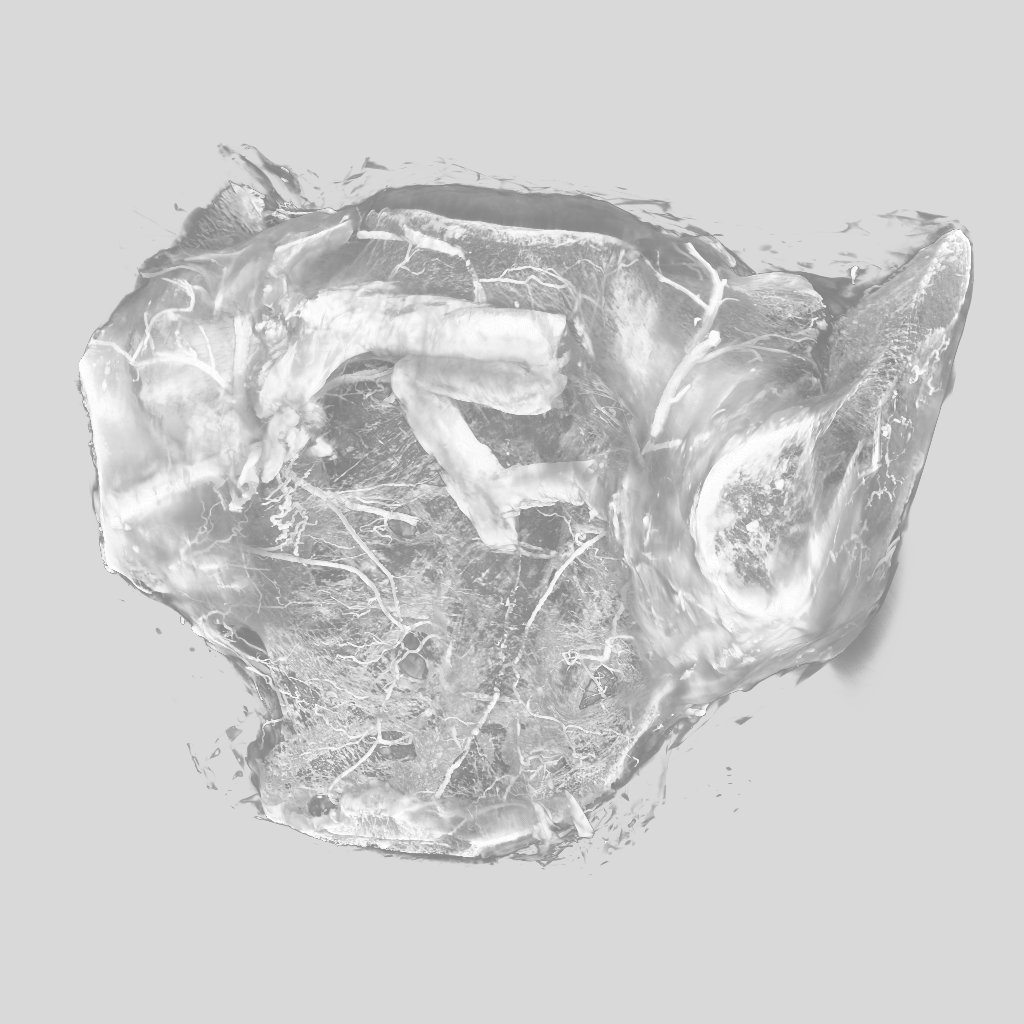
\includegraphics[width=\imagewidth]{./images/Halm/Becken/Sakrum_C/frames/video-0000}};
				% 723.669px = 160.034942115mm -> 100px = 22114.394um -> 2.261px = 500um, 0.452px = 100um
				\draw[|-|,white,thick,shadowed] (77,366) -- (797,436) node [sloped,midway,above] {\shadowtext{\SI{16}{\centi\meter}}};
			\end{tikzpicture}%
			}%
		\only<2>{%
			\animategraphics[palindrome,height=\imheight,every=\everyframe]{24}{./images/Halm/Becken/Sakrum_C/frames/video-0}{000}{101}%
			}
\end{frame}

% Fishes EAWAG
% Fishec	FieldID	OtherID	ReplacementID	FishID_ColourScanStatus	Length(cm)	TemporaryJar	Genus	Species	Ecology	Replicates
% 103754				103754	6.2		Yssichromis (core)	pyrrhocephalus	zooplanktivore	TZ 2010 MG transect
% 161543				161543 - reconstruct	17	Mark6	Harpagochromis	cf. pachycephalus	piscivore	TZ 2017	
%\begin{frame}[label=current]
%	\frametitle{Cichlids}
%	       \centering
%            % # Fish 161543, Scan head_30um_rec was scanned with 30 um
%            % For the visualization, we binned the stack 2x, thus have a voxel size of 60 um
%    	    % The image is 1412 pixels high, so we used `python ~/P/Dev/latex/draw_a_scalebar.py -p 12 -i frames/video-0000.jpg -l 1412` to draw a scale bar
%            \only<1>{%
%            \tikzset{shadowed/.style={preaction={transform canvas={shift={(1pt,-1pt)}},draw=ubRed, thick}}} % shadowed drawing https://tex.stackexchange.com/a/185853/828
%            \renewcommand{\imwidth}{\imheight/600*1024}%% My script breaks if we have a set image height. The movie frames are 1024x600, so we just calculate a new imwidth :)
%            \pgfmathsetlength{\imagewidth}{\imwidth}%
%            \pgfmathsetlength{\imagescale}{\imagewidth/1024}%
%            \def\x{633-50}% scalebar-x starting at golden ratio of image width of 1024px = 633
%            \def\y{540}% scalebar-y at 90% of image height of 600px = 540
%            \begin{tikzpicture}%
%            =\imagescale,y=-\imagescale]
%		        \node[anchor=north west, inner sep=0pt, outer sep=0pt] at (0,0) {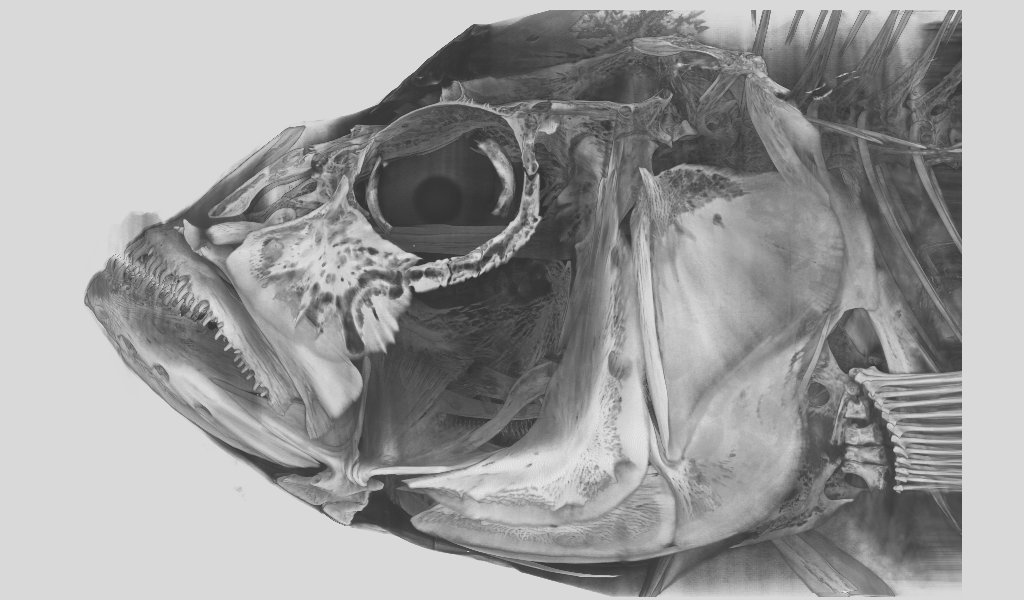
\includegraphics[width=\imagewidth]{./images/EAWAG/161543/head_30um/frames/video-0000}};
%	            %\spy [red] on (724,300) in node at (0,0) [anchor=north west];
%	            % 586.337px = 88.08mm -> 100px = 15022.075um -> 3.328px = 500um, 0.666px = 100um
%	            %\draw[|-|,blue,thick] (955,6) -- (960,592) node [sloped,midway,above,fill=white,semitransparent,text opacity=1] {\SI{88.08}{\milli\meter} (586px) TEMPORARY!};
%	            \draw[|-|,white,thick,shadowed] (\x,\y) -- (\x+332.8,\y) node [midway,above] {\shadowtext{\SI{5}{\centi\meter}}};
%            \end{tikzpicture}%
%            }%    	    
%%	        \only<2>{%
%%		        \animategraphics[height=\imheight,every=\everyframe]{24}{./images/EAWAG/161543/head_30um/frames/video-0}{000}{075}%
%%	    	}%
%%            \only<3>{%
%%		        \animategraphics[height=\imheight,every=\everyframe]{24}{./images/EAWAG/161543/head_30um/frames/video-0}{075}{240}%
%%		    }%	    	
%	    %\only<3>{%
%	    %    \animategraphics<3>[autoplay,height=\imheight,every=\everyframe]{24}{./images/EAWAG/161543/head_30um/frames/video-0}{241}{320}%
%	    %    }
%\end{frame}

\begin{frame}
	\frametitle{Cichlids}
	    \centering
	    % # Fish 103754, Scan head_rec was scanned with 12 um.
	    % The image is 1412 pixels high, so we used `python ~/P/Dev/latex/draw_a_scalebar.py -p 12 -i frames/video-0000.jpg -l 1412` to draw a scale bar
%	    \only<1>{%
            \renewcommand{\imwidth}{\imheight/600*1024}%% My script breaks if we have a set image height. The movie frames are 1024x600, so we just calculate a new imwidth :)
	            \tikzset{shadowed/.style={preaction={transform canvas={shift={(1pt,-1pt)}},draw=ubRed, thick}}}% shadowed drawing https://tex.stackexchange.com/a/185853/828
                \pgfmathsetlength{\imagewidth}{\imwidth}%
                \pgfmathsetlength{\imagescale}{\imagewidth/1024}%
                \def\x{633}% scalebar-x starting at golden ratio of image width of 1024px = 633
                \def\y{540}% scalebar-y at 90% of image height of 600px = 540
	            \begin{tikzpicture}[x=\imagescale,y=-\imagescale]
                    \node[anchor=north west, inner sep=0pt, outer sep=0pt] at (0,0) {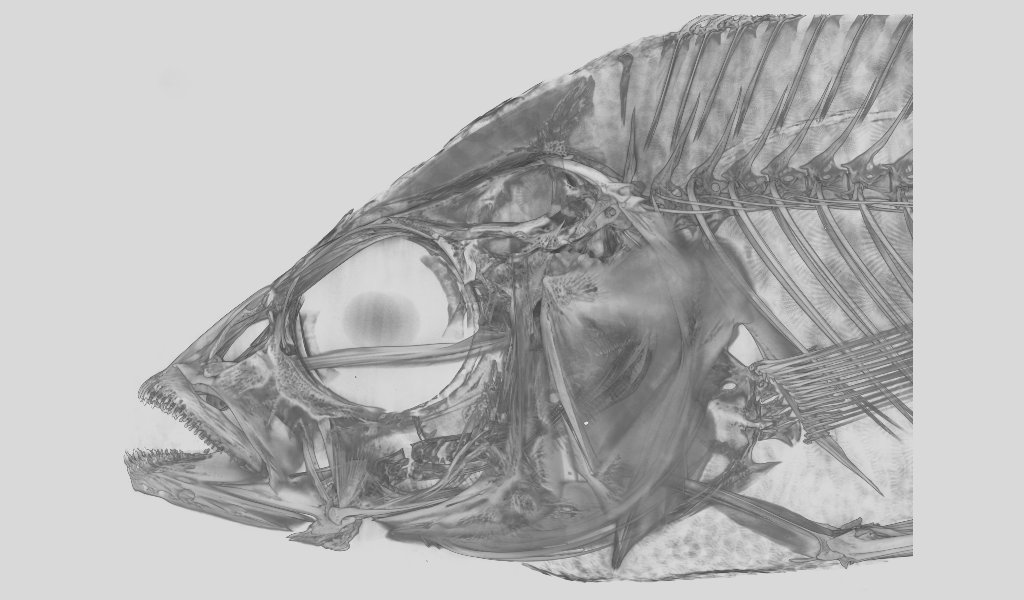
\includegraphics[width=\imagewidth]{./images/EAWAG/103754/head/frames/video-0000}};
                    % 538.843px = 16.944mm -> 100px = 3144.517um -> 15.901px = 500um, 3.180px = 100um
	                %\draw[|-|,blue,thick] (912,14) -- (910,553) node [sloped,midway,above,fill=white,semitransparent,text opacity=1] {\SI{16.944}{\milli\meter} (539px) TEMPORARY!};
	                \draw[|-|,white,thick,shadowed] (\x,\y) -- (\x+159.01,\y) node [midway,above] {\shadowtext{\SI{500}{\micro\meter}}};
                \end{tikzpicture}%
%            }%
%	    \only<2>{%
%	        \animategraphics[height=\imheight,every=\everyframe]{24}{./images/EAWAG/103754/head/frames/video-0}{000}{075}
%	    }%
%	%\only<2>{%
%	%    \animategraphics<2>[autoplay,height=\imheight,every=\everyframe]{24}{./images/EAWAG/103754/head/frames/video-0}{075}{240}%
%	%    }%
%	%\only<3>{%
%	%    \animategraphics<3>[autoplay,height=\imheight,every=\everyframe]{24}{./images/EAWAG/103754/head/frames/video-0}{241}{320}%
%	%    }%
\end{frame}

\renewcommand{\imwidth}{0.75\linewidth}
\renewcommand{\imheight}{0.618\paperheight}
\begin{frame}
	\frametitle{Teeeth}
	\begin{columns}
		\begin{column}{0.5\linewidth}
			\begin{itemize}
				\item<1-> 104 extracted human permanent mandibular canines									\item<2-> Root canal morphology, according to~\citeauthor{Briseno-Marroquin2015}~\cite{Briseno-Marroquin2015}
				\item<3-> \emph{Reproducible} analysis~\cite{Haberthur2020a}			\end{itemize}
		\end{column}
		\begin{column}{0.5\linewidth}
			\only<1>{%
				\centering
				\pgfmathsetlength{\imagewidth}{\imwidth}%
				\pgfmathsetlength{\imagescale}{\imagewidth/2716}%
				\def\x{1678}% scalebar-x starting at golden ratio of image width of 2716px = 1678
				\def\y{2444}% scalebar-y at 90% of image height of 2716px = 2444
				\begin{tikzpicture}[x=\imagescale,y=-\imagescale]
					\node[anchor=north west, inner sep=0pt, outer sep=0pt] at (0,0) {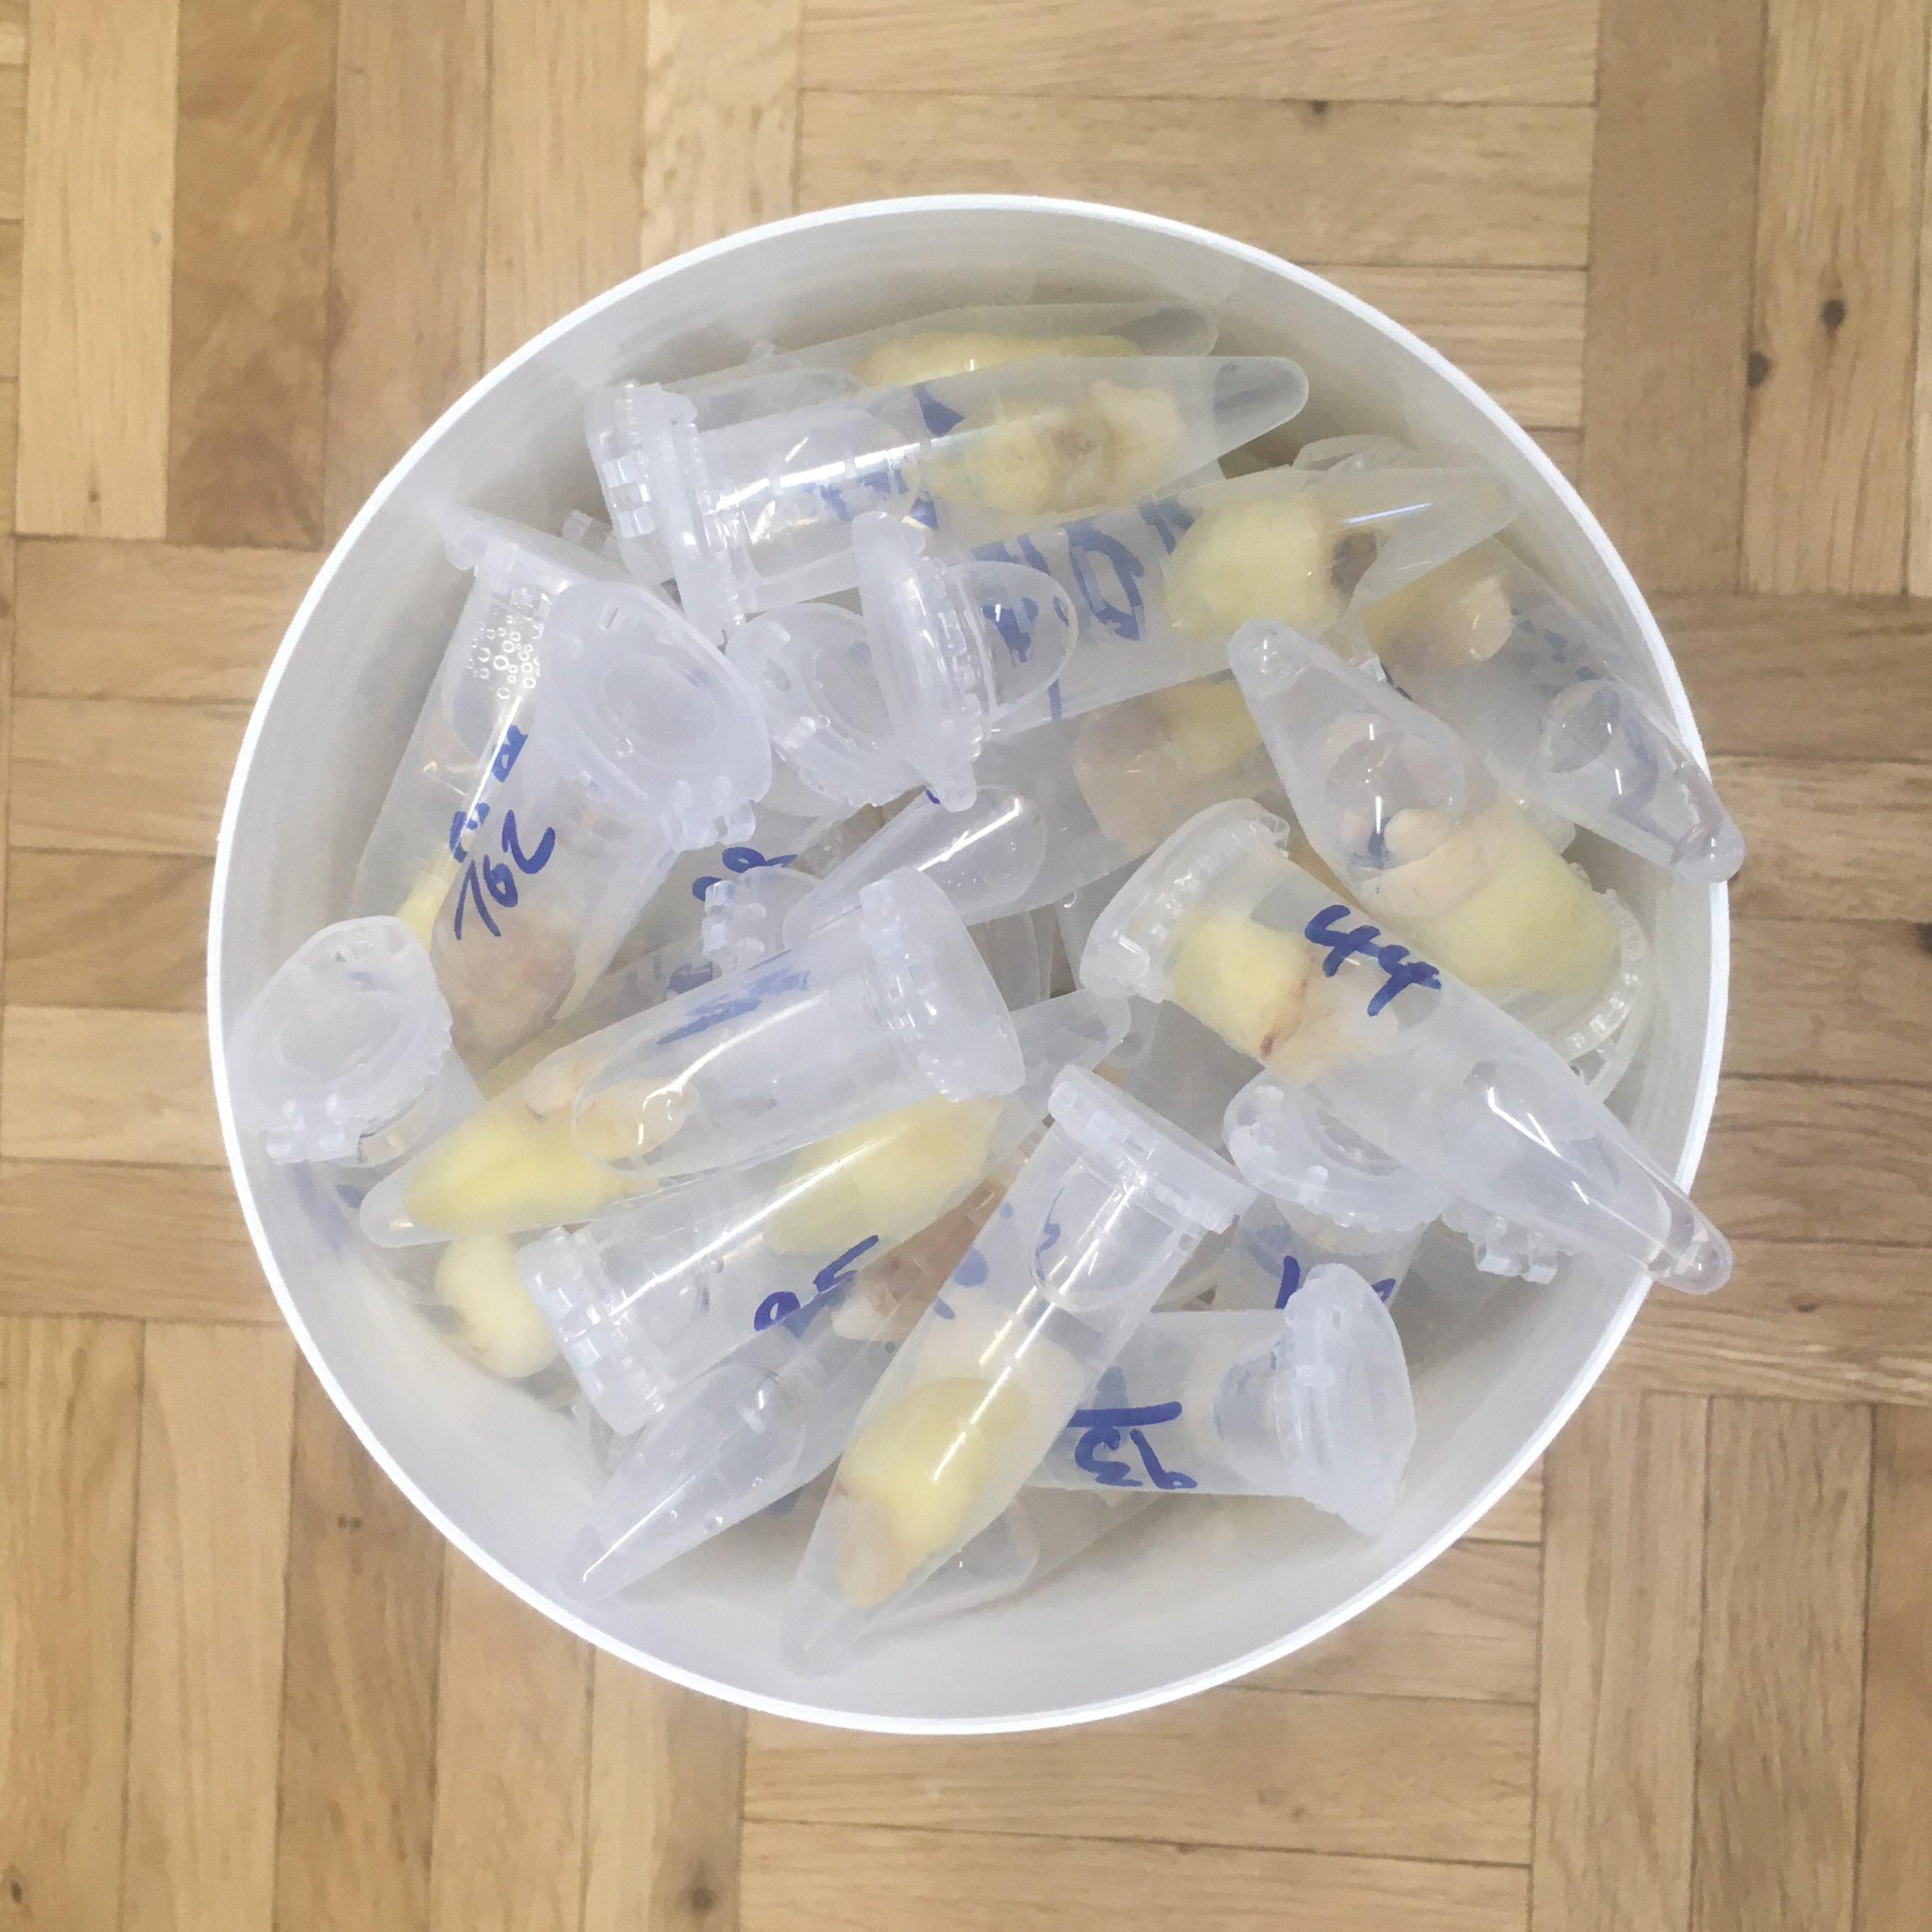
\includegraphics[width=\imagewidth]{./images/ZMK/bucketofteeth}};
					% 2132.087px = 140.0mm -> 100px = 6566.337um -> 7.615px = 500um, 1.523px = 100um
					%\draw[|-|,blue,thick] (299,1340) -- (2430,1406) node [sloped,midway,above,fill=white,semitransparent,text opacity=1] {\SI{140.0}{\milli\meter} (2132px) TEMPORARY!};
					\draw[|-|,white,thick,shadowed] (\x,\y) -- (\x+761.5,\y) node [midway,above] {\shadowtext{\SI{5}{\centi\meter}}};
				\end{tikzpicture}%
				}%
			\renewcommand{\imwidth}{\linewidth}%
			\only<2>{%
				\centering%
				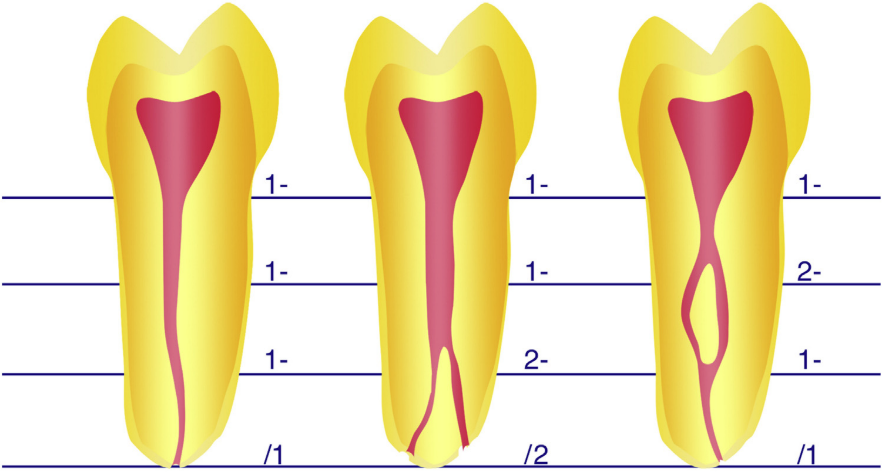
\includegraphics[width=\imwidth]{./images/ZMK/briseno}%
				\sourcecite{Briseno-Marroquin2015}{Fig.~2}%
				}%
			\only<3>{%
				\centering
				%\href{https://mybinder.org/v2/gh/habi/zmk-tooth-cohort/master?filepath=ToothAnalysis.ipynb}{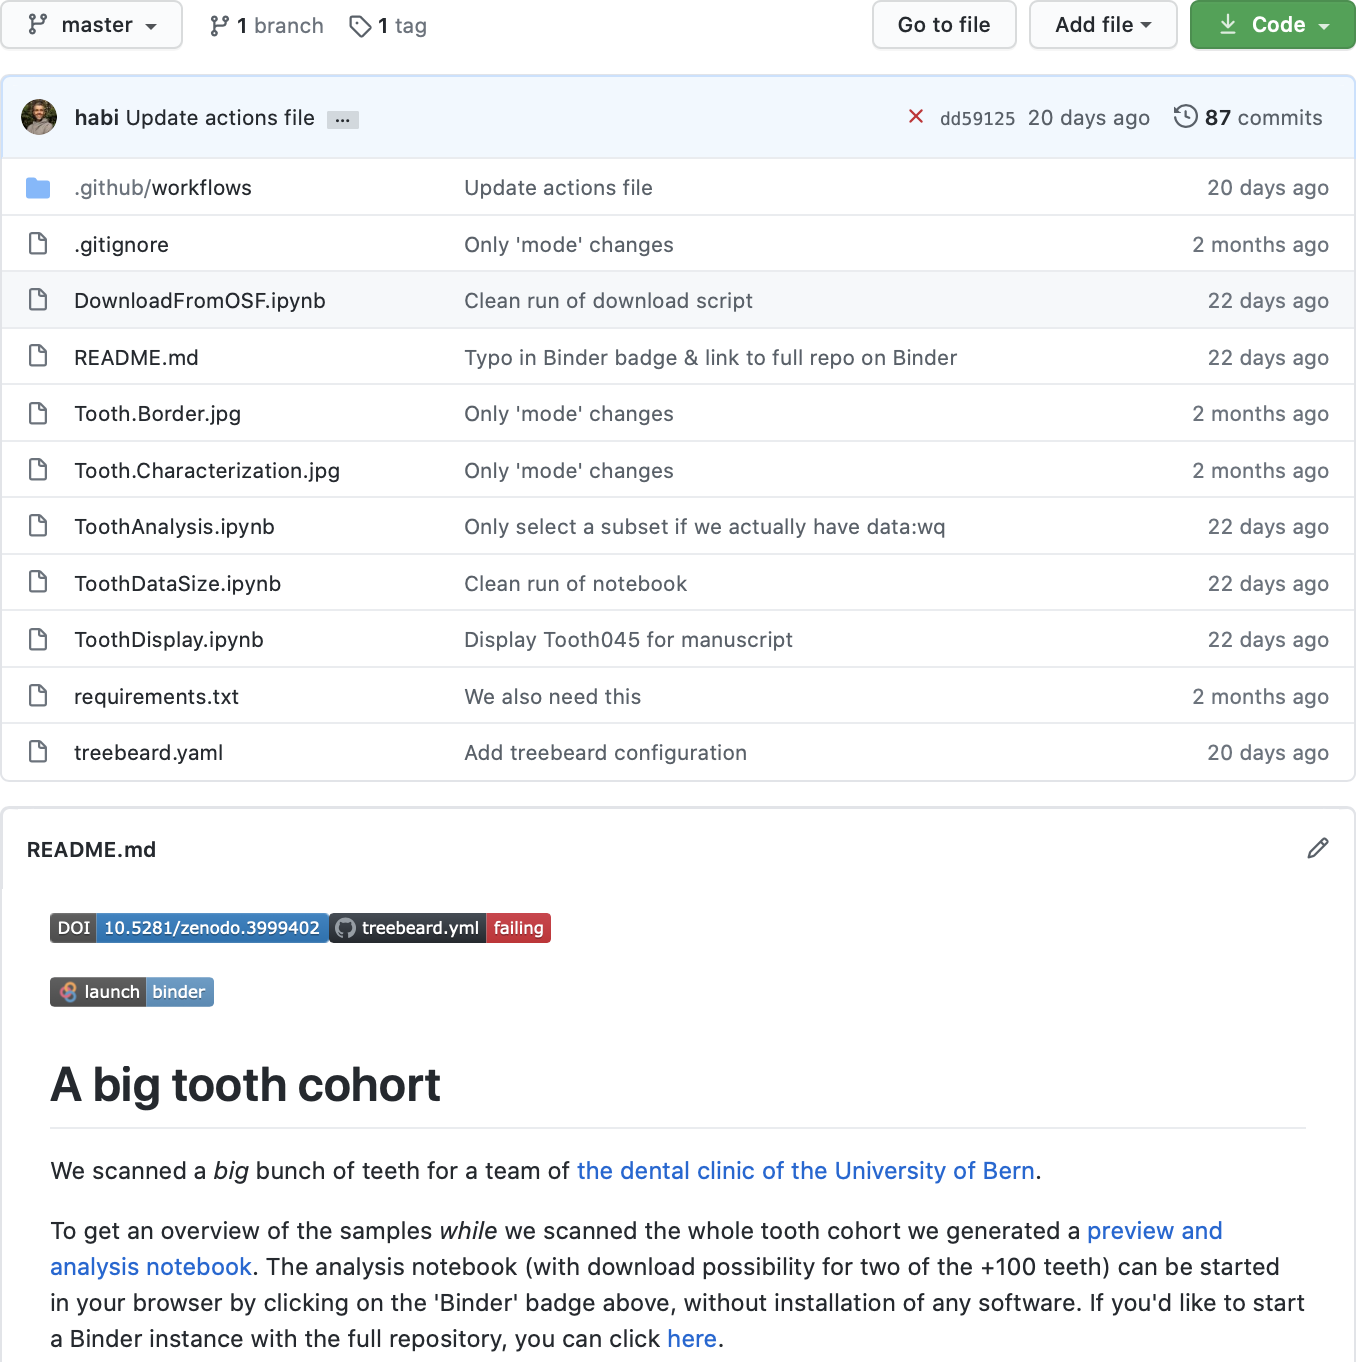
\includegraphics[height=\imheight]{./images/binder}}%
				}%
		\end{column}
	\end{columns}
\end{frame}

\begin{frame}
	\frametitle{Tooth morphology}
	\begin{tikzpicture}[remember picture,overlay]%
		\node at (current page.center) [shift={(0,-25pt)}]{%
			\only<1>{\animategraphics[autoplay,loop,width=\paperwidth,every=\everyframe]{24}{./images/ZMK/tooth045/full/image0}{000}{474}}%
			\only<2>{\animategraphics[autoplay,loop,width=\paperwidth,every=\everyframe]{24}{./images/ZMK/tooth045/full-slices/image0}{000}{466}}%
			};%
	\end{tikzpicture}%
\end{frame}

\begin{frame}
	\frametitle{Extraction of root canal space}
	\begin{tikzpicture}[remember picture,overlay]%
	\node at (current page.center) [shift={(0,-25pt)}]{%
		\only<1>{\animategraphics[autoplay,loop,width=\paperwidth,every=\everyframe]{24}{./images/ZMK/tooth045/transparent-slices/image0}{000}{473}}%
		\only<2>{\animategraphics[autoplay,loop,width=\paperwidth,every=\everyframe]{24}{./images/ZMK/tooth045/transparent-slices-pulpa/image0}{000}{457}}%
		%\only<3>{\animategraphics[autoplay,loop,width=\paperwidth,every=\everyframe]{24}{./images/ZMK/tooth045/pulpa/image0}{000}{413}}%
		};%
	\end{tikzpicture}%
\end{frame}


\begin{frame}[label=current]
	\frametitle{Meteorite Chrondrules}
%Reset image height

\renewcommand{\imwidth}{0.725\paperheight}% set global image height
% Scaled Image Pixel Size (um)=0.399990
% We used a binned dataset for the visualization, e.g. the voxel size is 0.79998 um
% The diameter of the chondrule is ~1263 voxels, so we used `python ~/P/Dev/latex/draw_a_scalebar.py -p 0.79998 -i frames/video-0000.jpg -l 1236` to generate a scale bar for both views.

%%----------
\tikzset{shadowed/.style={preaction={transform canvas={shift={(1pt,-1pt)}},draw=green, thick}}} % shadowed drawing https://tex.stackexchange.com/a/185853/828
\pgfmathsetlength{\imagewidth}{\imwidth}%
\pgfmathsetlength{\imagescale}{\imagewidth/1024}%
\def\x{633}% scalebar-x starting at golden ratio of image width of 1024px = 633
\def\y{922}% scalebar-y at 90% of image height of 1024px = 922
\begin{tikzpicture}[x=\imagescale,y=-\imagescale]
		\node[anchor=north west, inner sep=0pt, outer sep=0pt] at (0,0) {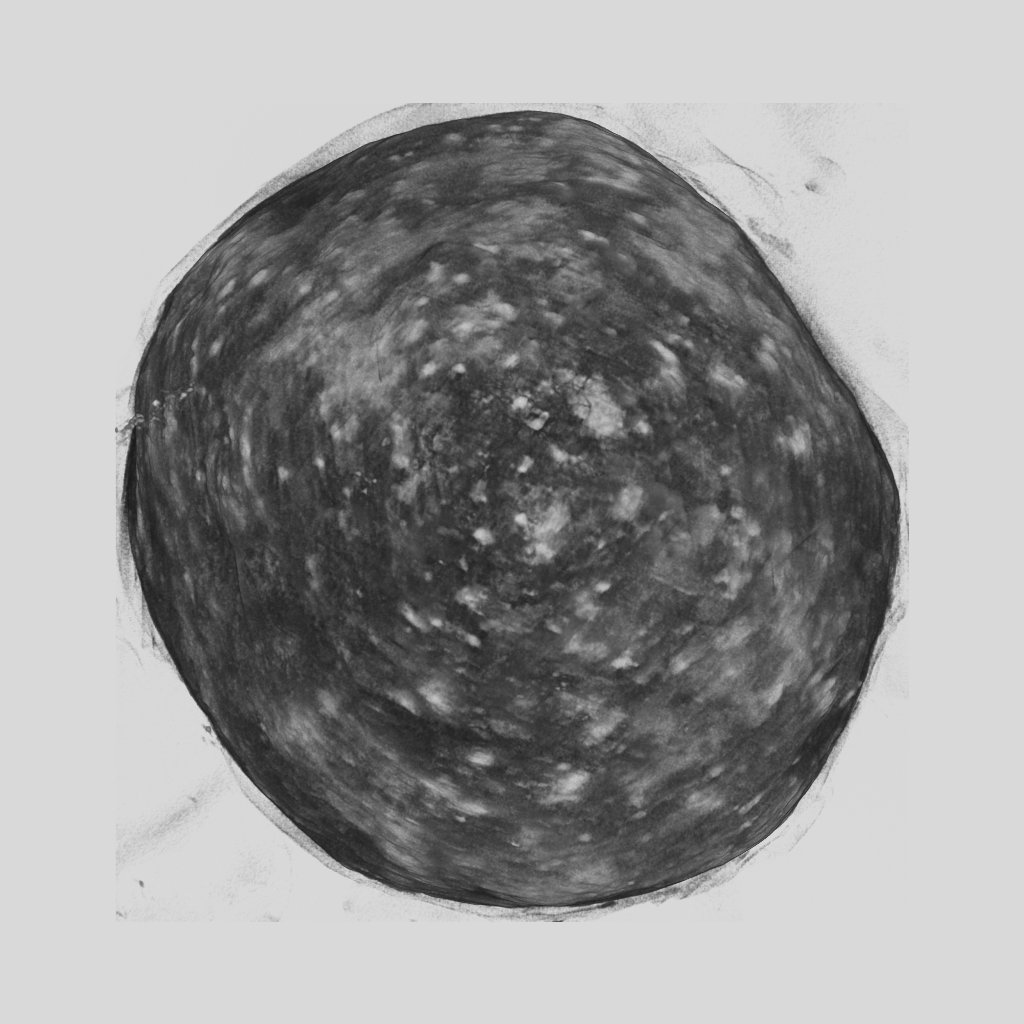
\includegraphics[width=\imagewidth]{./images/Chondrules Space Yogita/NWA1241_HR2/frames/video-0100}};
	% 815.741px = 0.98877528mm -> 100px = 121.212um -> 412.501px = 500um, 82.500px = 100um
	%\draw[|-|,blue,thick] (201,244) -- (802,796) node [sloped,midway,above,fill=white,semitransparent,text opacity=1] {\SI{0.98877528}{\milli\meter} (816px) TEMPORARY!};
	\draw[|-|,white,thick,shadowed] (\x,\y) -- (\x+412.501,\y) node [midway,above] {\shadowtext{\SI{500}{\micro\meter}}};
	%\draw[color=red, anchor=south west] (0,1024) node [fill=white, semitransparent] {Legend} node {Legend};
\end{tikzpicture}%
%%----------
\end{frame}

\begin{frame}[label=current]
	\frametitle{Meteorite Chrondrules}
        \centering
		\animategraphics[autoplay,height=\imheight,every=\everyframe]{24}{./images/"Chondrules Space Yogita"/NWA1241_HR2/frames/video-0}{000}{100}
\end{frame}

\begin{frame}
	\frametitle{Thanks}
	Images from us
	
	Werbung für Workshop: COMULIS Training School: \url{https://www.ana.unibe.ch/continuing_education/comulis_training_school/}
\end{frame}

\begin{frame}
	\frametitle{References}
	% Make the references continuously smaller :)
	%\renewcommand*{\bibfont}{\small}
	%\renewcommand*{\bibfont}{\footnotesize}
	%\renewcommand*{\bibfont}{\scriptsize}
	%\renewcommand*{\bibfont}{\tiny}
%	\setbeamertemplate{bibliography item}{\insertbiblabel}
	\printbibliography
\end{frame}

\end{document}
